\documentclass[aspectratio=169, 10pt]{beamer}

\usetheme{metropolis}
\metroset{block=fill, numbering=fraction, progressbar=frametitle}

\usepackage[utf8]{inputenc}
\usepackage[T1]{fontenc}
\usepackage[spanish]{babel}
\usepackage{graphicx}
\usepackage{amsmath, amssymb}
\usepackage{booktabs}
\usepackage{xcolor}

\graphicspath{{../ej2/results/}{../extra/results/}}

\definecolor{accent}{HTML}{0F4C81}
\setbeamercolor{frametitle}{bg=accent}
\setbeamercolor{progress bar}{fg=accent}

\renewcommand{\maketitle}{\frame{\titlepage}}

\title{Variational Autoencoders}
\subtitle{TP5 --- EJ2 sobre emojis 16x16}
\author{Sistemas de Inteligencia Artificial}
\institute{ITBA --- 2026}
\date{\today}

\begin{document}

\maketitle

\begin{frame}{Del AE al VAE}
  \begin{columns}[T]
    \begin{column}{0.42\textwidth}
      \begin{itemize}
        \item En EJ1 el AE reconstruye bien.
        \item Pero su latente \textbf{no} esta pensado para muestrear.
        \item Generar desde coordenadas nuevas puede caer en zonas sin estructura.
      \end{itemize}
      \vspace{0.5em}
      \begin{block}{Idea}
        El VAE agrega el termino KL para empujar el latente hacia
        $\mathcal{N}(0,I)$ y volverlo \textbf{sampleable}.
      \end{block}
    \end{column}
    \begin{column}{0.58\textwidth}
      \centering
      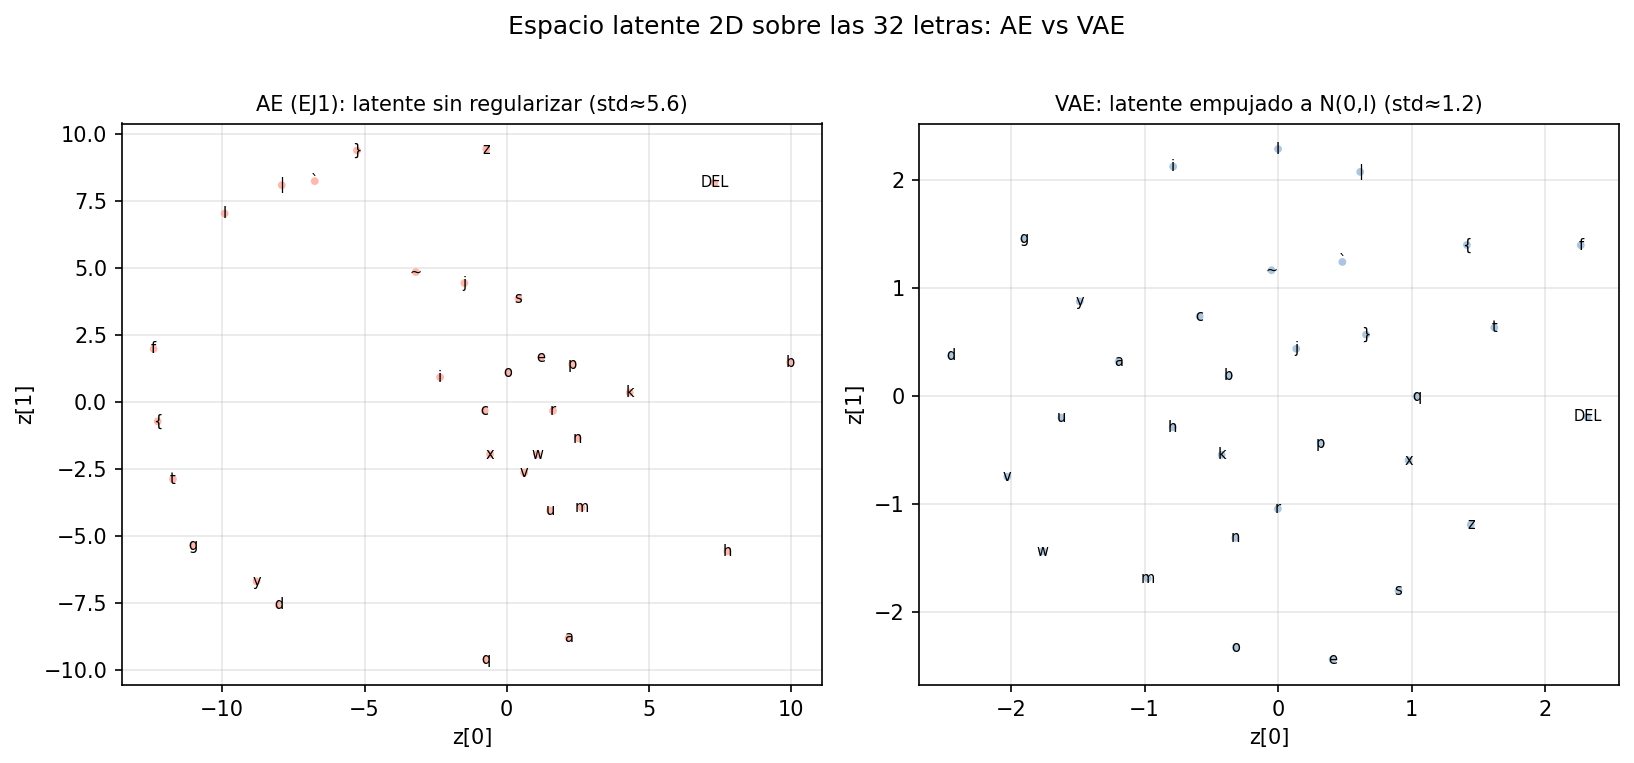
\includegraphics[width=0.95\linewidth]{letters_ae_vs_vae_scatter.png}
    \end{column}
  \end{columns}
\end{frame}

\begin{frame}{El problema y el nuevo dataset}
  \begin{columns}[T]
    \begin{column}{0.45\textwidth}
      \begin{table}\small
        \begin{tabular}{ll}
          \toprule
          Dataset & \texttt{emojis.npz} \\
          Resolucion & \textbf{16x16} en grises \\
          Input & \textbf{256} pixeles \\
          Muestras & \textbf{960} \\
          Clases & \textbf{16} \\
          \bottomrule
        \end{tabular}
      \end{table}
      \vspace{0.5em}
      \textbf{Pregunta gancho}: \emph{\textbf{podemos aprender un espacio latente
      desde el cual generar emojis nuevos plausibles?}}

      \vspace{0.5em}
      \begin{block}{Objetivo del EJ2}
        Aprender un VAE tal que:
        \[
          z \sim \mathcal{N}(0,I) \Longrightarrow decoder(z)
        \]
        produzca muestras nuevas que parezcan pertenecer al dataset.
      \end{block}
    \end{column}
    \begin{column}{0.55\textwidth}
      \centering
      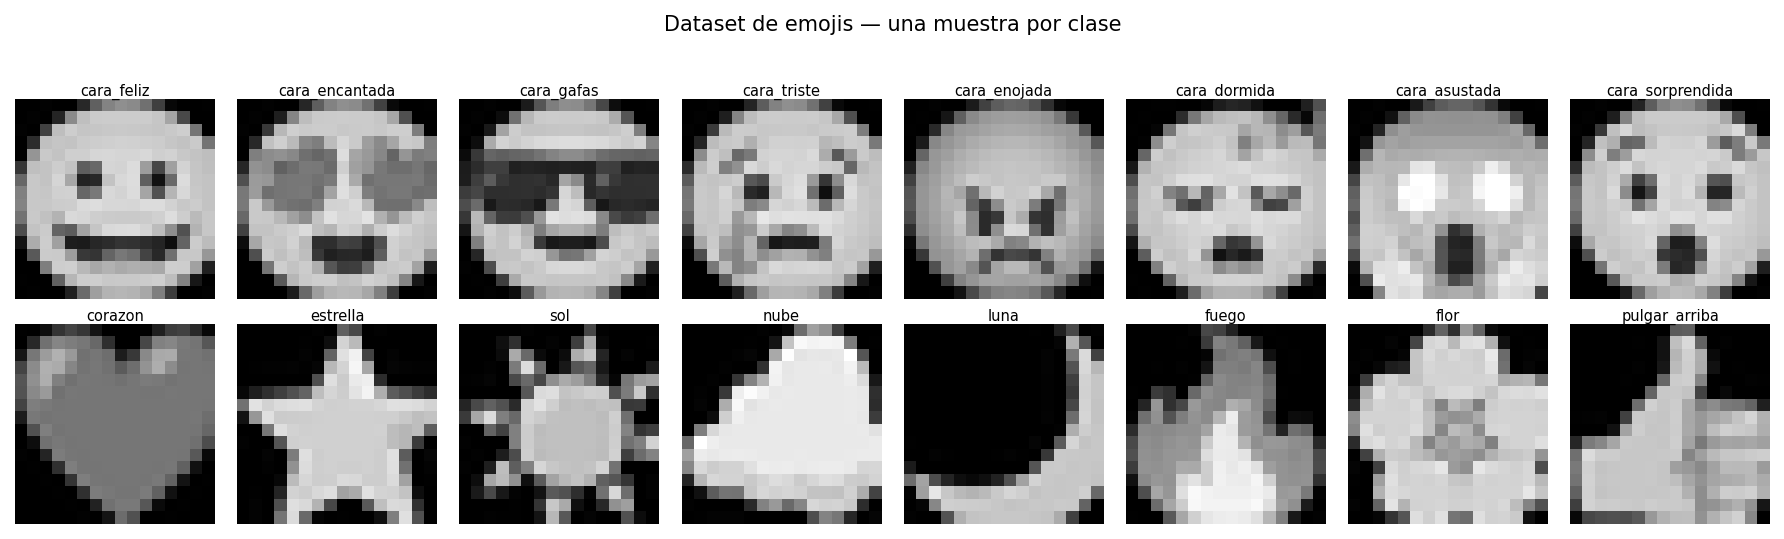
\includegraphics[width=0.95\linewidth]{dataset_sample.png}
    \end{column}
  \end{columns}
\end{frame}

\begin{frame}{Arquitectura base y parametros a estudiar}
  \begin{columns}[T]
    \begin{column}{0.53\textwidth}
      Encoder variacional + decoder:
      \[
        x \in \mathbb{R}^{256} \to [256,64] \to (\mu, \log\sigma^2)
      \]
      \[
        z = \mu + \sigma \odot \varepsilon, \qquad \varepsilon \sim \mathcal{N}(0,I)
      \]
      \[
        z \to [64,256] \to \hat{x}
      \]
      \vspace{0.3em}
      \[
        \mathcal{L} = BCE(x,\hat{x}) + \beta\,KL(q(z\mid x)\Vert\mathcal{N}(0,I))
      \]
      \vspace{0.3em}
      \begin{itemize}
        \item \textbf{BCE}: fuerza reconstruccion.
        \item \textbf{KL}: ordena el latente cerca de $\mathcal{N}(0,I)$.
        \item Esta es la \emph{configuracion base}; despues variamos una pieza a la vez.
      \end{itemize}
    \end{column}
    \begin{column}{0.47\textwidth}
      \begin{table}\scriptsize
        \begin{tabular}{ll}
          \toprule
          Encoder / Decoder & $[256,64]$ / $[64,256]$ \\
          Activacion oculta & ReLU \\
          Salida & logistica \\
          Optimizador & Adam \\
          Batch / Epocas & $64$ / $600$ \\
          Seed & $42$ \\
          \midrule
          \textit{Parametros a elegir} & $\beta$, $latent\_dim$, \\
                                        & recon loss, warmup \\
          \bottomrule
        \end{tabular}
      \end{table}
      \vspace{0.4em}
      Gradient-check del backward:\\
      error relativo max \textbf{$1.25\times 10^{-10}$}.
    \end{column}
  \end{columns}
\end{frame}

\begin{frame}{Eje 1 --- Peso del KL: $\beta$-VAE}
  \centering
  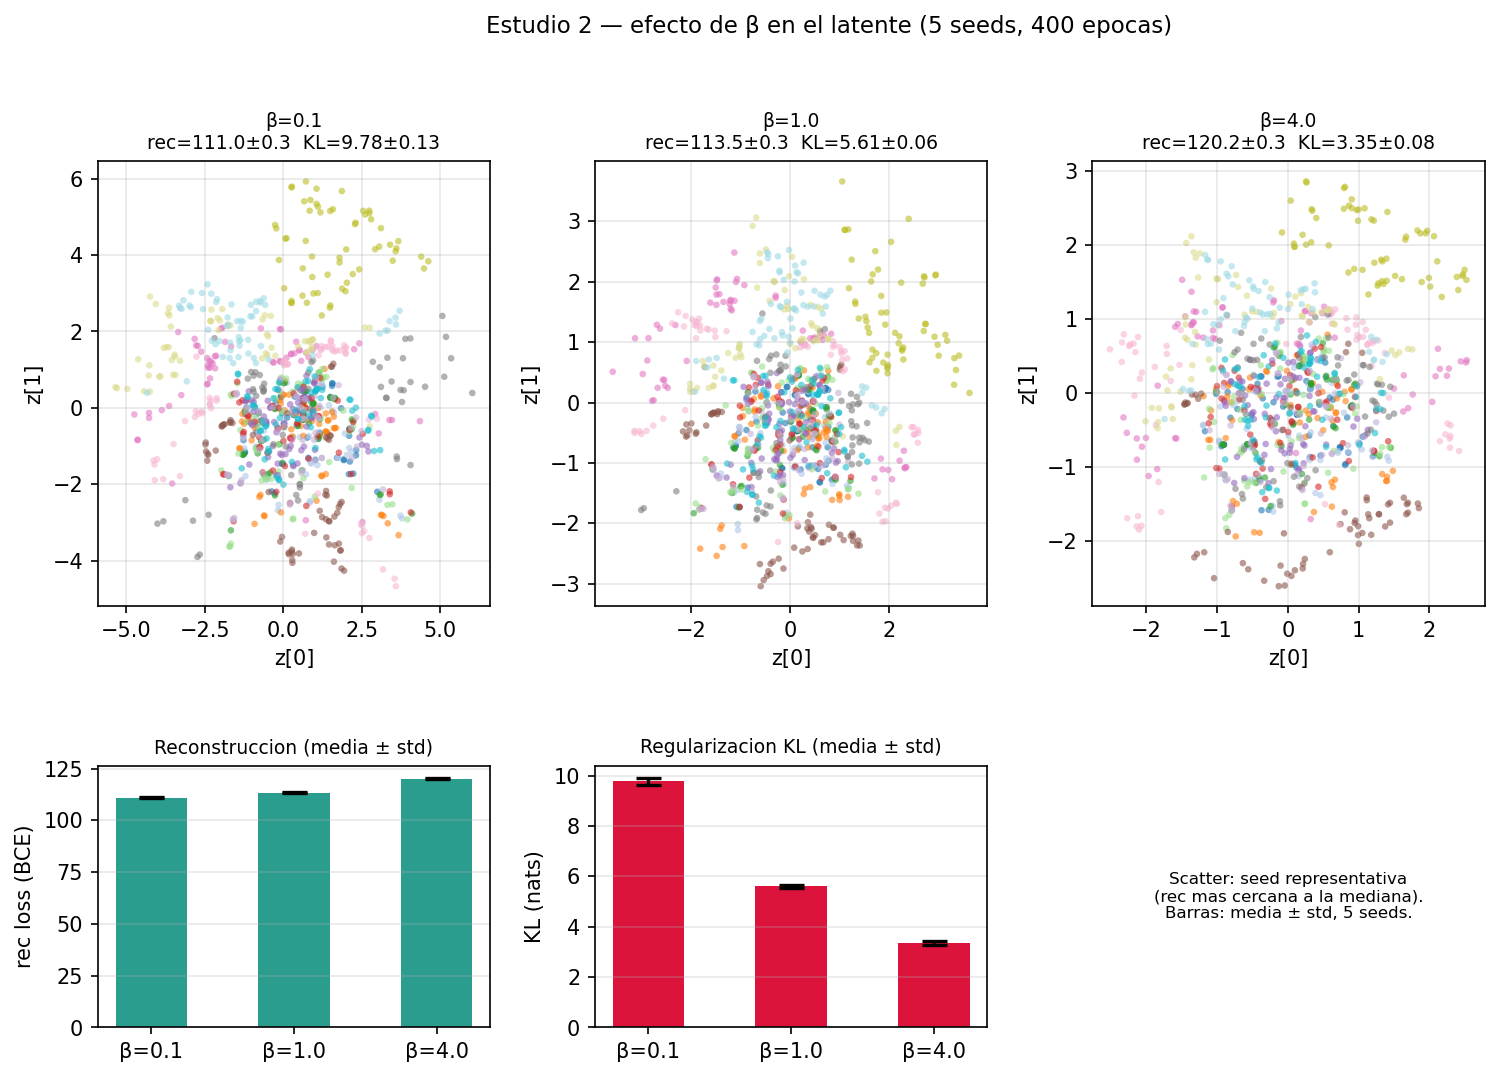
\includegraphics[width=0.95\linewidth]{exp_beta.png}
  \vfill
  {\footnotesize $\beta=0.1$: mejor reconstruccion, menos regularizacion.
  $\beta=4$: latente mas forzado, peor detalle.\; \textbf{Elegimos $\beta=1$}
  como compromiso entre reconstruccion y estructura latente.}
\end{frame}

\begin{frame}{Eje 2 --- Generacion desde el prior}
  \begin{columns}[T]
    \begin{column}{0.36\textwidth}
      \begin{block}{Punto (c) del enunciado}
        Para generar \textbf{no usamos el encoder}.
        \[
          z \sim \mathcal{N}(0,I)
          \quad \Longrightarrow \quad
          decoder(z)
        \]
      \end{block}
      Estas imagenes son \textbf{muestras nuevas}, no inputs del dataset.
    \end{column}
    \begin{column}{0.64\textwidth}
      \centering
      
\includegraphics[width=0.92\linewidth]{samples.png}
    \end{column}
  \end{columns}
\end{frame}

\begin{frame}{Eje 3 --- Dentro vs fuera del prior}
  \centering
  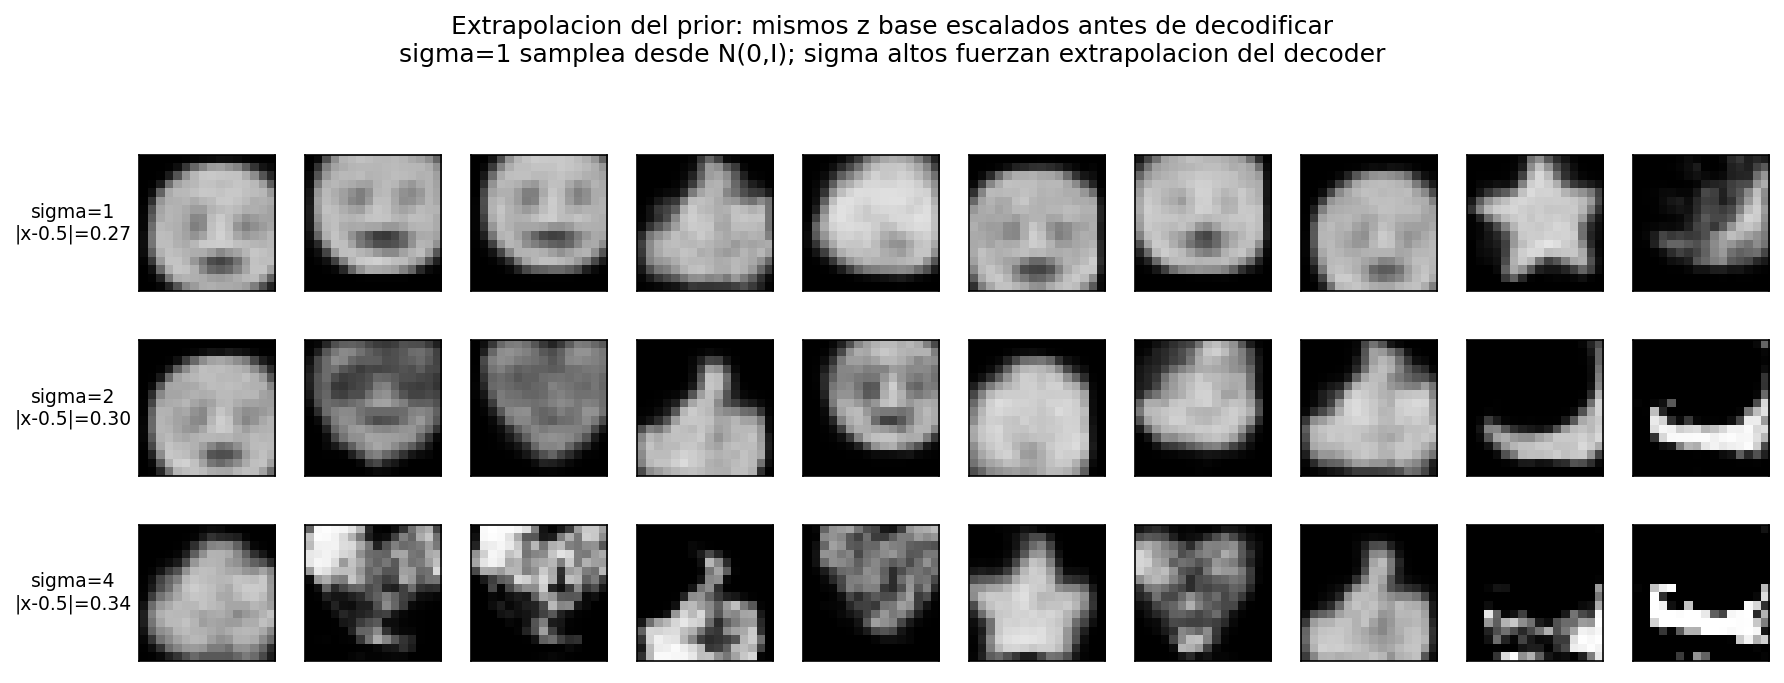
\includegraphics[width=0.92\linewidth]{exp_prior_extrapolation.png}
  \vfill
  {\footnotesize $\sigma=1$ samplea desde el prior. Al escalar $z$ con
  $\sigma=2$ y $4$ nos alejamos de la region donde el decoder fue entrenado por
  el KL.\; \textbf{La generacion debe evaluarse cerca de $\mathcal{N}(0,I)$.}}
\end{frame}

\begin{frame}{Eje 4 --- Dimension latente}
  \begin{columns}[T]
    \begin{column}{0.58\textwidth}
      \centering
      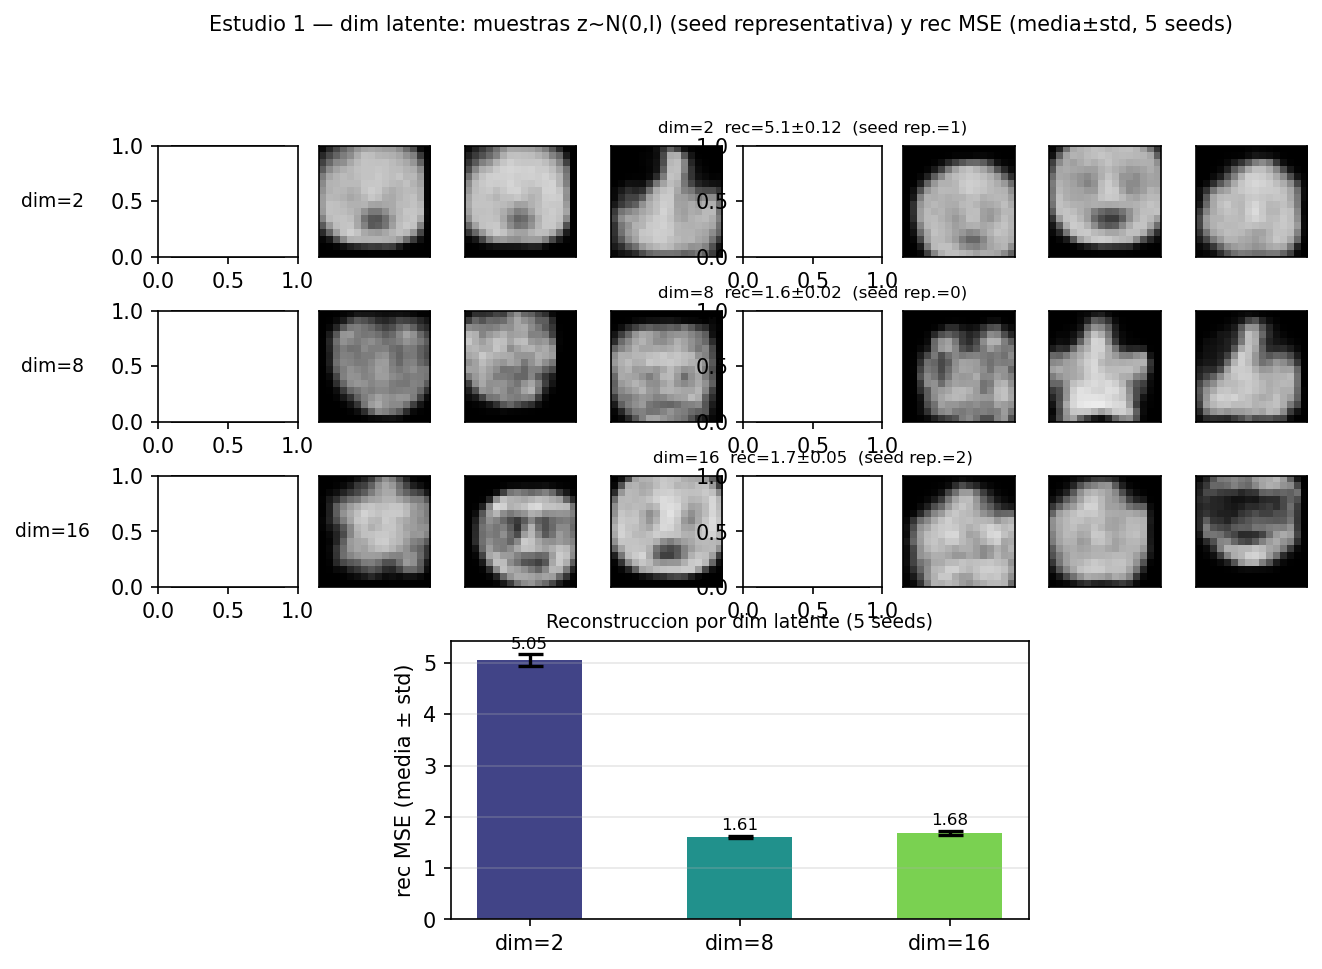
\includegraphics[width=\linewidth]{exp_latent_dim.png}
    \end{column}
    \begin{column}{0.42\textwidth}
      \begin{itemize}
        \item 2D: interpretable, pero limitado.
        \item 8D: gran mejora de reconstruccion.
        \item 16D: mejora marginal extra.
      \end{itemize}
      \vspace{0.5em}
      rec\_MSE:
      \begin{itemize}
        \item 2D: 5.27
        \item 8D: 1.61
        \item 16D: 1.63
      \end{itemize}
      \textbf{Decision:} 2D para visualizar, >2D para capacidad.
    \end{column}
  \end{columns}
\end{frame}

\begin{frame}{Eje extra --- BCE vs MSE}
  \centering
  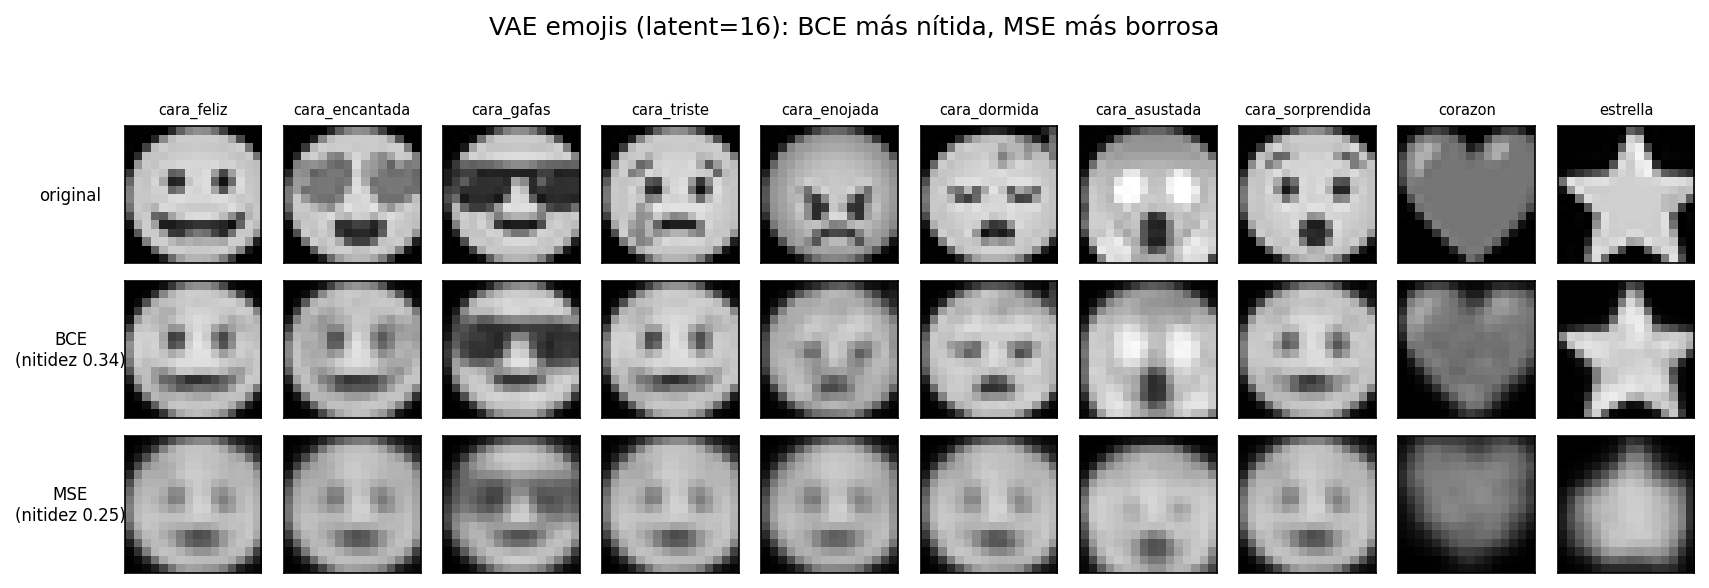
\includegraphics[width=0.95\linewidth]{recon_loss_mse_vs_bce.png}
  \vfill
  {\footnotesize Dos VAE identicos salvo la loss de reconstruccion.
  \textbf{BCE} queda mas nitida y ademas reconstruye mejor:
  rec\_MSE \textbf{1.38} vs \textbf{5.22}.\; \textbf{Fijamos BCE}.}
\end{frame}

\begin{frame}{Eje extra --- \textquestiondown memoriza o generaliza?}
  \begin{columns}[T]
    \begin{column}{0.58\textwidth}
      \centering
      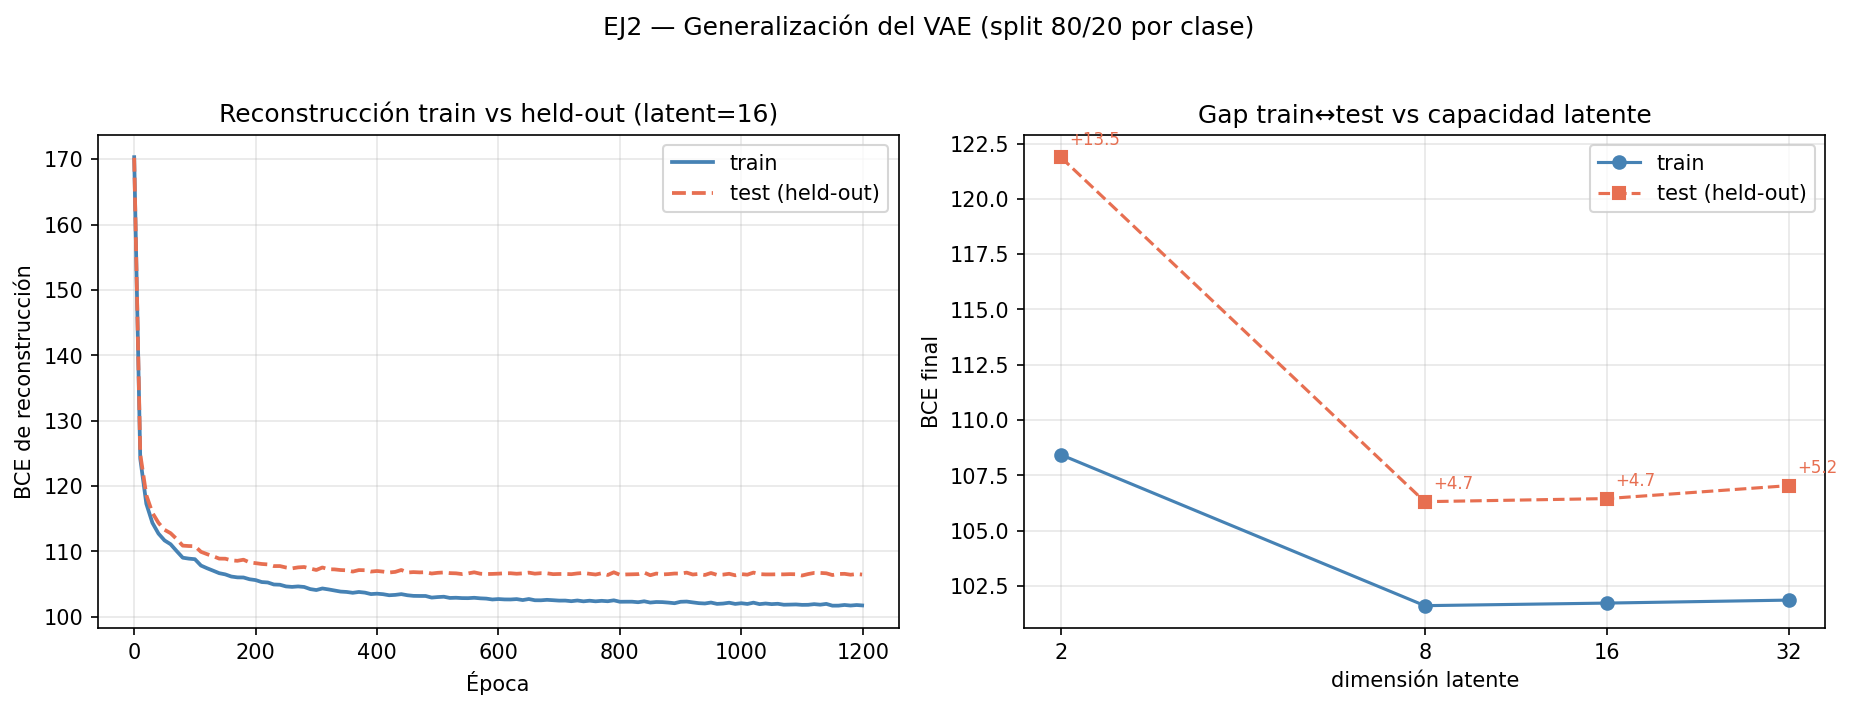
\includegraphics[width=\linewidth]{generalization_curves.png}
    \end{column}
    \begin{column}{0.42\textwidth}
      Split 80/20 por clase.
      \vspace{0.5em}
      \begin{itemize}
        \item Latente 2D underfitea.
        \item Para 8/16/32 el gap train-test queda acotado.
      \end{itemize}
      \vspace{0.4em}
      Gap final:
      \begin{itemize}
        \item 2D: +13.46
        \item 8D: +4.70
        \item 16D: +4.73
        \item 32D: +5.18
      \end{itemize}
    \end{column}
  \end{columns}
\end{frame}

\begin{frame}{Reconstruccion del modelo final}
  \begin{columns}[T]
    \begin{column}{0.35\textwidth}
      Corrida principal:
      \begin{itemize}
        \item latente 2D
        \item BCE
        \item $\beta=1$
        \item Adam
        \item 600 epocas
      \end{itemize}
      \vspace{0.4em}
      Final:
      \begin{itemize}
        \item total: 117.995
        \item rec: 112.219
        \item KL: 5.776
        \item rec\_MSE: 4.576
      \end{itemize}
    \end{column}
    \begin{column}{0.65\textwidth}
      \centering
      
\includegraphics[width=0.94\linewidth]{reconstructions.png}
    \end{column}
  \end{columns}
\end{frame}

\begin{frame}{Espacio latente 2D}
  \begin{columns}[T]
    \begin{column}{0.58\textwidth}
      \centering
      
\includegraphics[width=0.95\linewidth]{latent_scatter.png}
    \end{column}
    \begin{column}{0.42\textwidth}
      Cada punto es el \textbf{$\mu(x)$} de un emoji.
      \vspace{0.5em}
      \begin{itemize}
        \item La reconstruccion separa informacion relevante.
        \item El KL evita que los codigos se dispersen arbitrariamente.
      \end{itemize}
      \vspace{0.4em}
      Lo importante no es separar perfecto, sino que el espacio sea
      \textbf{compacto y sampleable}.
    \end{column}
  \end{columns}
\end{frame}

\begin{frame}{Manifold generativo e interpolacion}
  \begin{columns}[T]
    \begin{column}{0.54\textwidth}
      \centering
      
\includegraphics[height=0.60\textheight]{manifold_grid.png}
    \end{column}
    \begin{column}{0.46\textwidth}
      \centering
      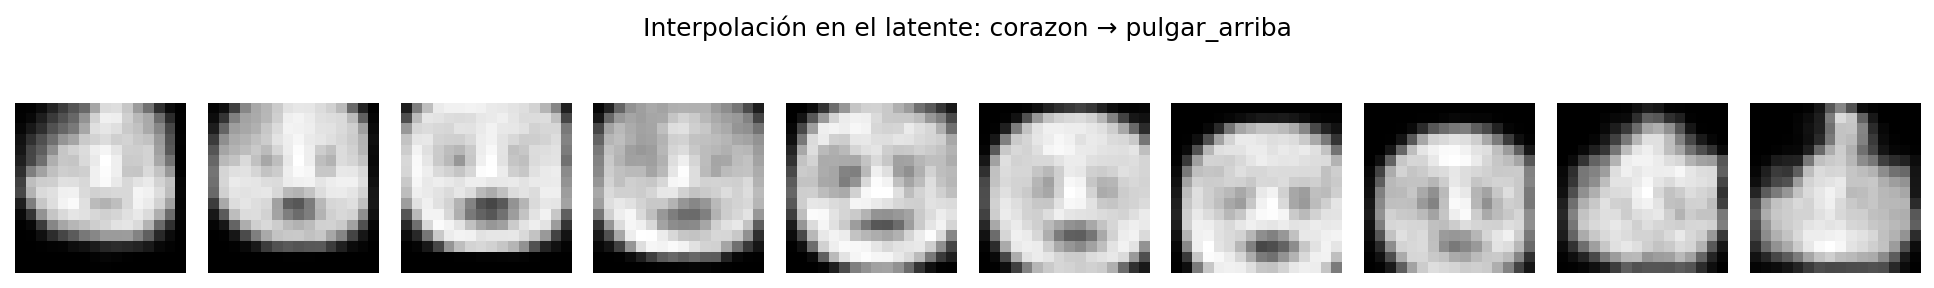
\includegraphics[width=\linewidth]{interpolation.png}\\[0.3em]
      {\scriptsize El decoder aprende una funcion continua $z\to imagen$.
      Pequenos movimientos en el latente producen cambios graduales.}
    \end{column}
  \end{columns}
\end{frame}

\begin{frame}{Corrida larga: 600 vs 50k epocas}
  \centering
  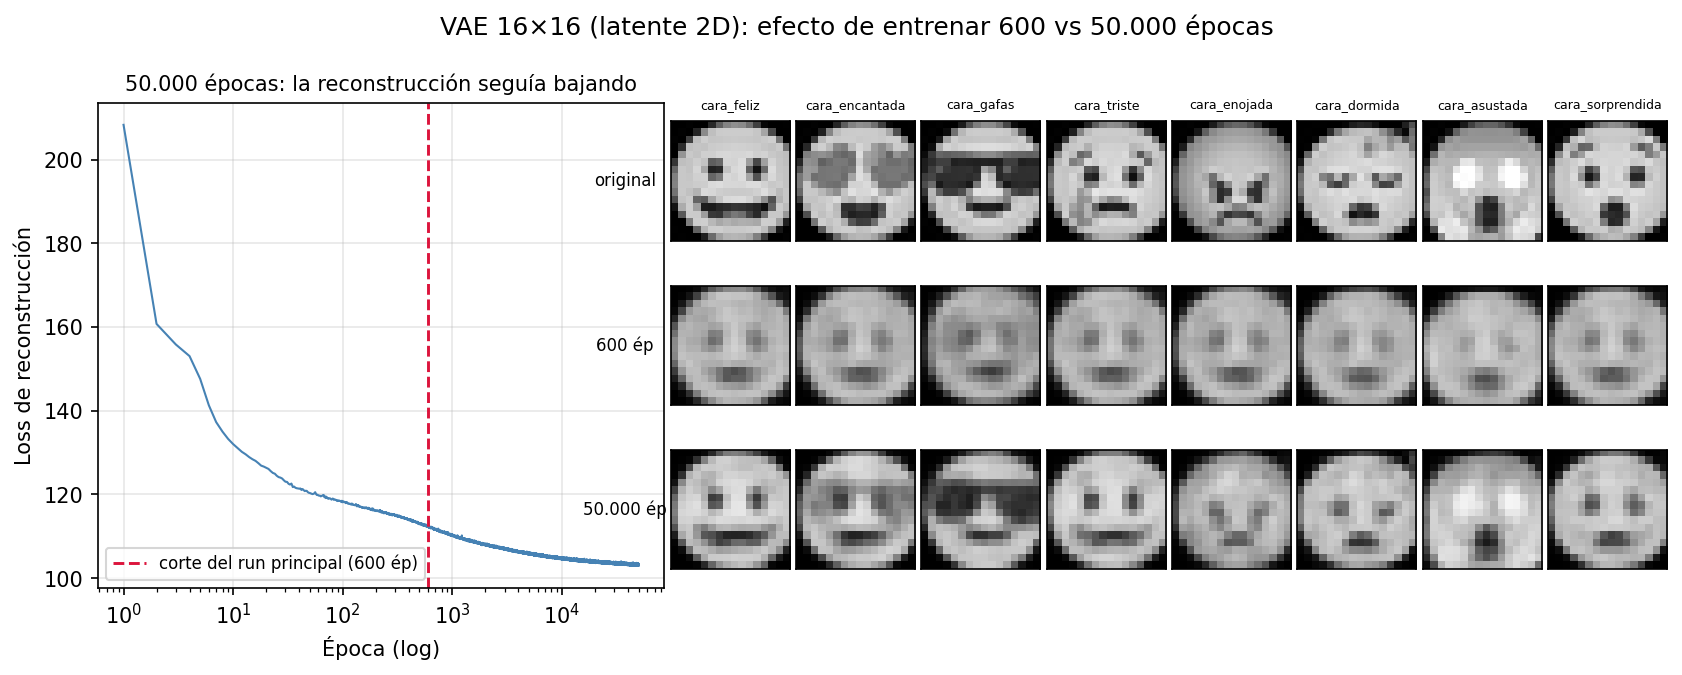
\includegraphics[width=0.95\linewidth]{comparison_600_vs_50k.png}
  \vfill
  {\footnotesize Entrenar mas mejora detalle, pero no cambia la conclusion
  central: el aporte del VAE es \textbf{ordenar el latente para poder samplear}.}
\end{frame}

\begin{frame}{Conclusiones}
  \begin{itemize}
    \item Un AE puede reconstruir sin tener un latente generativo.
    \item El VAE agrega una regularizacion probabilistica via KL.
    \item Eso permite generar con $z\sim\mathcal{N}(0,I)$.
    \item $\beta$ controla el trade-off entre reconstruccion y regularizacion.
    \item La generacion funciona sobre todo \textbf{dentro} de la region del prior.
    \item Mas dimension latente no siempre implica mas informacion util.
  \end{itemize}
\end{frame}

\end{document}
